\documentclass[12pt]{article}
\usepackage{graphicx}
\usepackage{amsfonts}
\usepackage{amsmath}
\usepackage{amssymb}
\usepackage{enumitem}
\usepackage{xcolor}

\usepackage[a4paper, margin=1in]{geometry}

\setlength{\headheight}{15pt}
\usepackage{fancyhdr}
\pagestyle{fancy}
\fancyhf{}
\fancyhead[L]{CPSC/EENG 420 - Lab Report 3}
\fancyhead[R]{Bryan SebaRaj  \thepage}

\linespread{1.3} 

\title{Lab 3: Superscalar PARCv2 Processor}
\author{Bryan SebaRaj \\[0.5em] Professor Abhishek Bhattacharjee \\[0.5em] EENG 420 - Computer Architecture}
\date{April 4, 2025}

\begin{document}

\maketitle

% Abstract: introductory paragraph summarizing the lab
% • Design: describe your implementation, justifications for design decisions (if any), deviations from the
% prescribed datapath, discussion of any extensions
% • Testing Methodology: describe how you tested the modules and your overall testing strategy–justify
% the effectiveness of your assembly test(s) in testing the functionality of the processor
% • Evaluation: report your simulation results and cycle counts
% • Discussion: comparison and analysis of benchmark results, discussion of tradeoffs of using bypassing
% over stalling
% • Figures: updated PARCv2 datapaths with bypassing and with bypassing and pipelined muldiv uni

\subsection*{Abstract}

\subsection*{Design}

\subsubsection*{Objective 1: Two-Wide Superscalar Processor with Dual Fetch, Single Issue}

\subsubsection*{Objective 2: Two-Wide Superscalar Processor}

\noindent No extensions were implemented.

\subsection*{Testing Methodology}


\subsection*{Evaluation}

The three versions of the pipelined processor were tested using the following
benchmarks: vector add, complex multiply, masked filter, and binary search. The
cycle counts and IPC for each benchmark are shown below in the format, cycle
count / IPC.

\begin{center}
    \begin{tabular}{|c || c | c | c|} 
 \hline
 Benchmark & pv2dualfetch & pv2ssc & pv2byp \\
 \hline\hline

 \hline

\end{tabular}
\end{center}

\subsection*{Discussion}

\subsection*{Figures}

\begin{center}
% 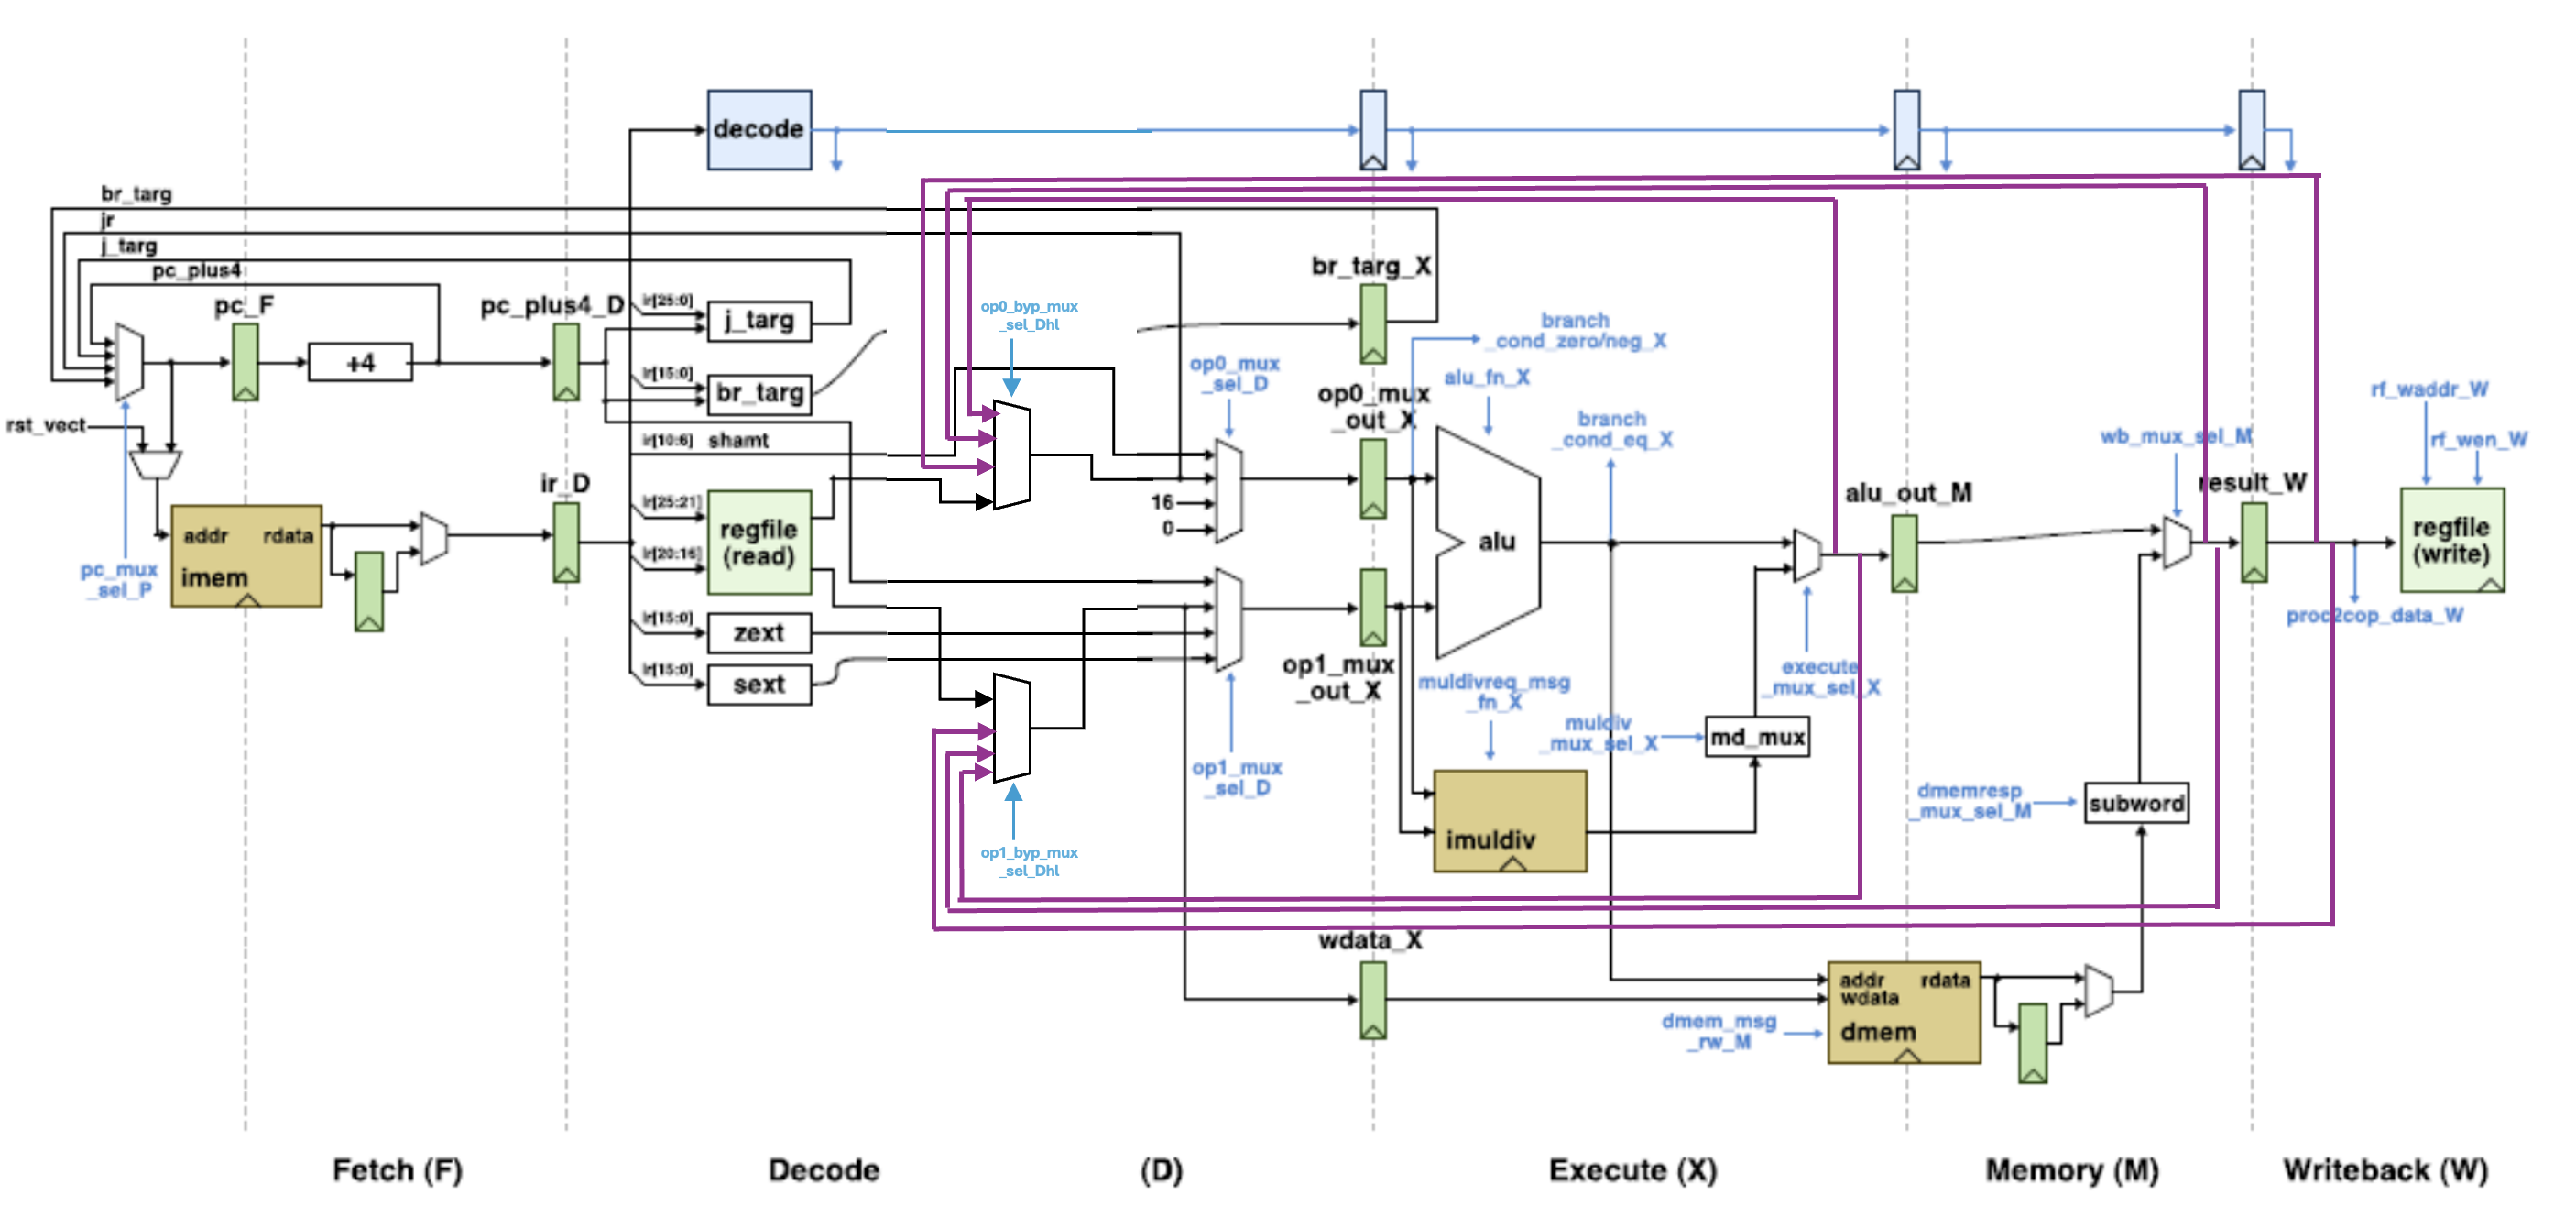
\includegraphics[scale=0.32]{../lab2_bypdpath.png}
% Figure 1: PARCv2 datapath with bypassing.
\end{center}

\vspace{0.3cm}
%See the new muxes within the Decode stage, one for op0 and one for op1. 

\begin{center}
% 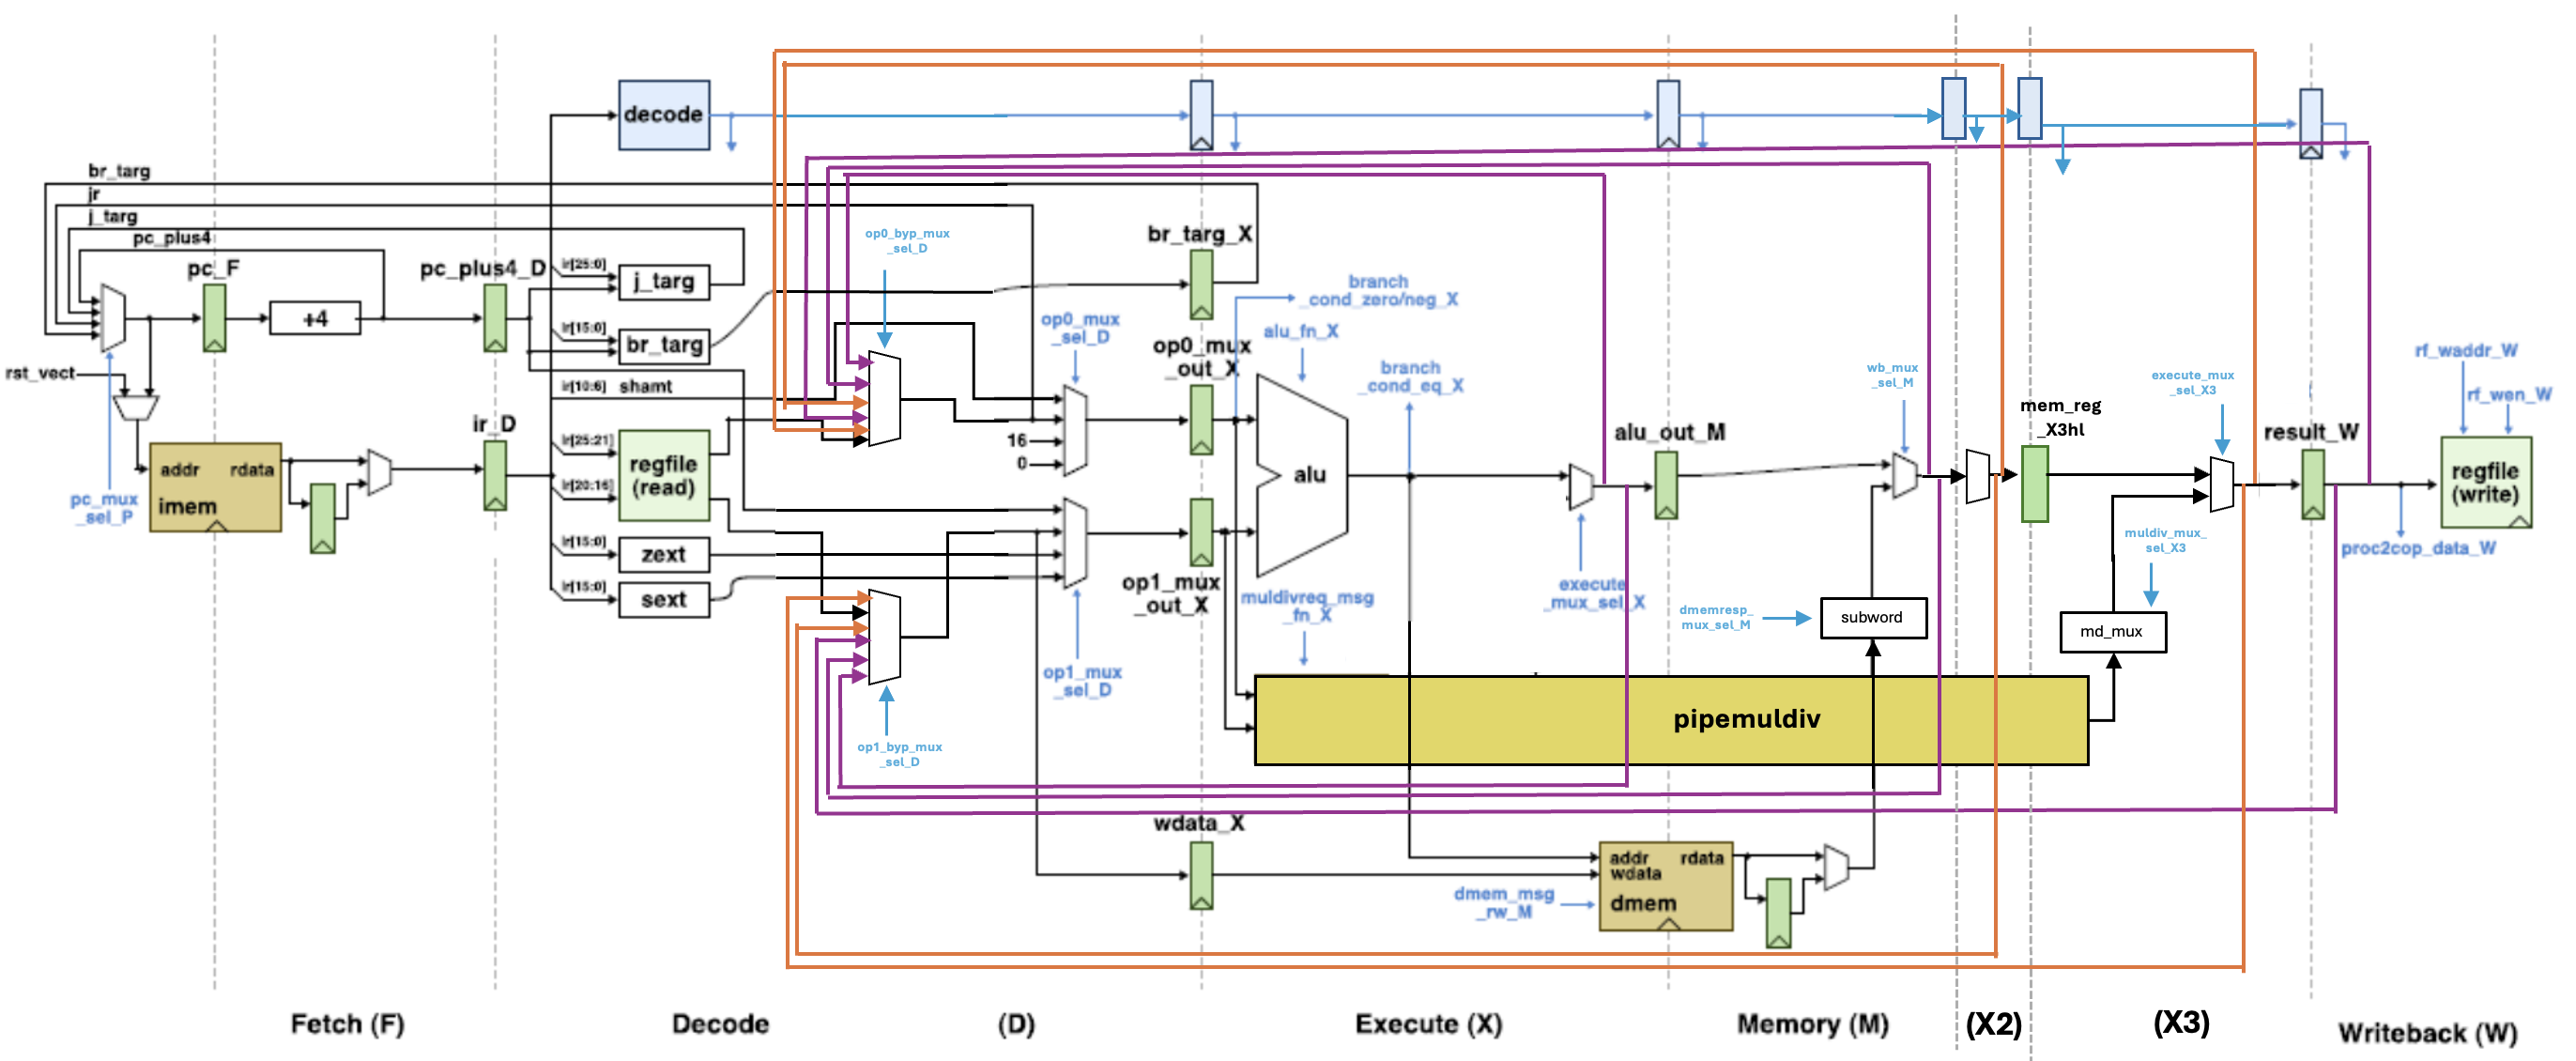
\includegraphics[scale=0.28]{../lab2_longdpath.png}
% Figure 2: PARCv2 datapath with pipelined muldiv unit, with appropriate stalling and bypassing. 
\end{center}



\end{document}


